\subsection{Der Master}
	Der Master ist die Person (unter den getrackten Personen), der es obliegt, die Anwendung zu steuern, d.\,h. in unserem Anwendungsfall der Präsentation ist der Master der Präsentierende.\par
	Es muss gewährleistet werden, dass nur der Master das Programm steuert und dabei von weiteren Personen im Raum nicht (bzw. nicht ohne weiteres) gestört werden kann. Die Erkennung muss robust gegen Jittering der Kinectdaten sein.\par
	Grundsätzlich kamen für die Festlegung des Masters zwei Ideen auf. Zunächst sollte bei jedem Frame, die getrackte Person, identifiziert werden, die der Kinect bzgl. der z-Koordinate am nähesten ist und diese als Master festgelegt werden. Der Master könnte hierbei bei jedem Frame zwischen den getrackten Personen wechseln. \par
	Die zweite Möglichkeit war die Festlegung des Masters auf eine bestimmte Person, von der zunächst bestimmte Identifikations-Merkmale eingespeichert werden und die dann anhand dieser als Master reidentifiziert werden kann. Sofern diese Festlegung erst einmal geschehen ist, bleibt diese Person Master, selbst nachdem sich diese zwischenzeitlich in einem ungetrackten Zustand (beispielsweise beim Herausgehen aus dem getrackten Bereich) befunden hat und dann wieder als getrackt erkannt wird. Bei einer Recherche, welche Merkmale sich aus den von der Kinect gelieferten Daten extrahieren lassen ließen, um hierfür in Frage zu kommen, stießen wir hierbei auf verschiedene Möglichkeiten, von denen einige jedoch aufgrund ihrer Unpraktikabilität ausschieden (Erkennung anhand des Gangs oder anhand der Stimme würde bei unserer Anwendung keinen Sinn machen, da die Master-Person während der Bedienung kaum umher läuft und diese hierfür nicht zu sprechen braucht). Schließlich stiessen wir auch auf Verfahren die die Skelettdaten der Kinect zur Identifikation nutzen. Dies schien die für unsere Zwecke praktikabelste Lösung zu sein, wenngleich unser Ansatz die Skelettdaten zu nutzen im Vergleich zu denjenigen in den gefundenen Arbeiten stark vereinfacht wurde.\par
	Grundlegendstes Prinzip für die Identifizierung einer Person ist hierbei das Auslesen der Skelettkoordinatenpunkte mit Hilfe des Kinect SDKs und daraus der Ermittlung diverser Längen als Körper proportionen mittels der Berechnung des euklidischen Abstands zwischen den entsprechenden Skelettpunkten. Beispielsweise wird die rechte Oberarmlänge als Abstand zwischen dem rechten Schulterpunkt und dem rechten Elbogenpunkt ermittelt. Weitere Körperproportionen die verwendet wurden sind unter anderem die Schulterbreite, Hüftbreite, Unterarmlänge, Abstand zwischen Hals und Kopf. \par

\begin{figure}
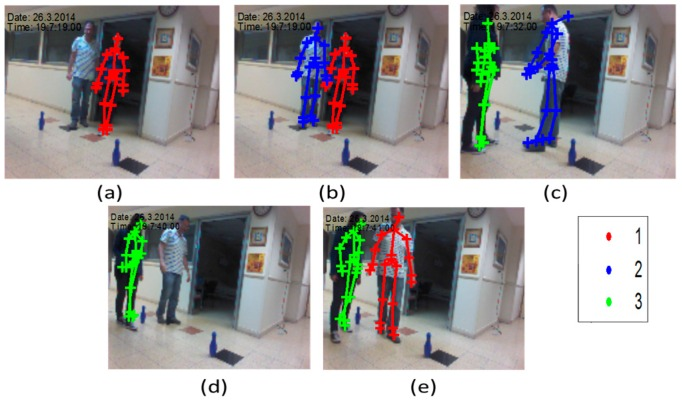
\includegraphics[width=\textwidth]{pictures/sensors-16-01965-g005.jpg}
\caption{Neuzuordnung von IDs nach zwischenzeitlichem \glqq Verlust\grqq{} von Skeletten, Quelle:\cite{bodyprop}}
\label{fig:fehlerk}
\end{figure}

Nach einigen Experimenten mit den Körperproportionen wurde festgestellt, dass einige Proportionen übermässig große Abweichungen aufwiesen, wenn die gleiche Person in unterschiedlichen Posen mit der Kinect vermessen wurde. (Beispielsweise die gemessene Schulterbreite, welche sich signifikant zwischen der Standard-Pose und einer Pose bei der die Arme über den Kopf gestreckt sind unterschied.) 
\begin{figure}[h!]
		\centering
		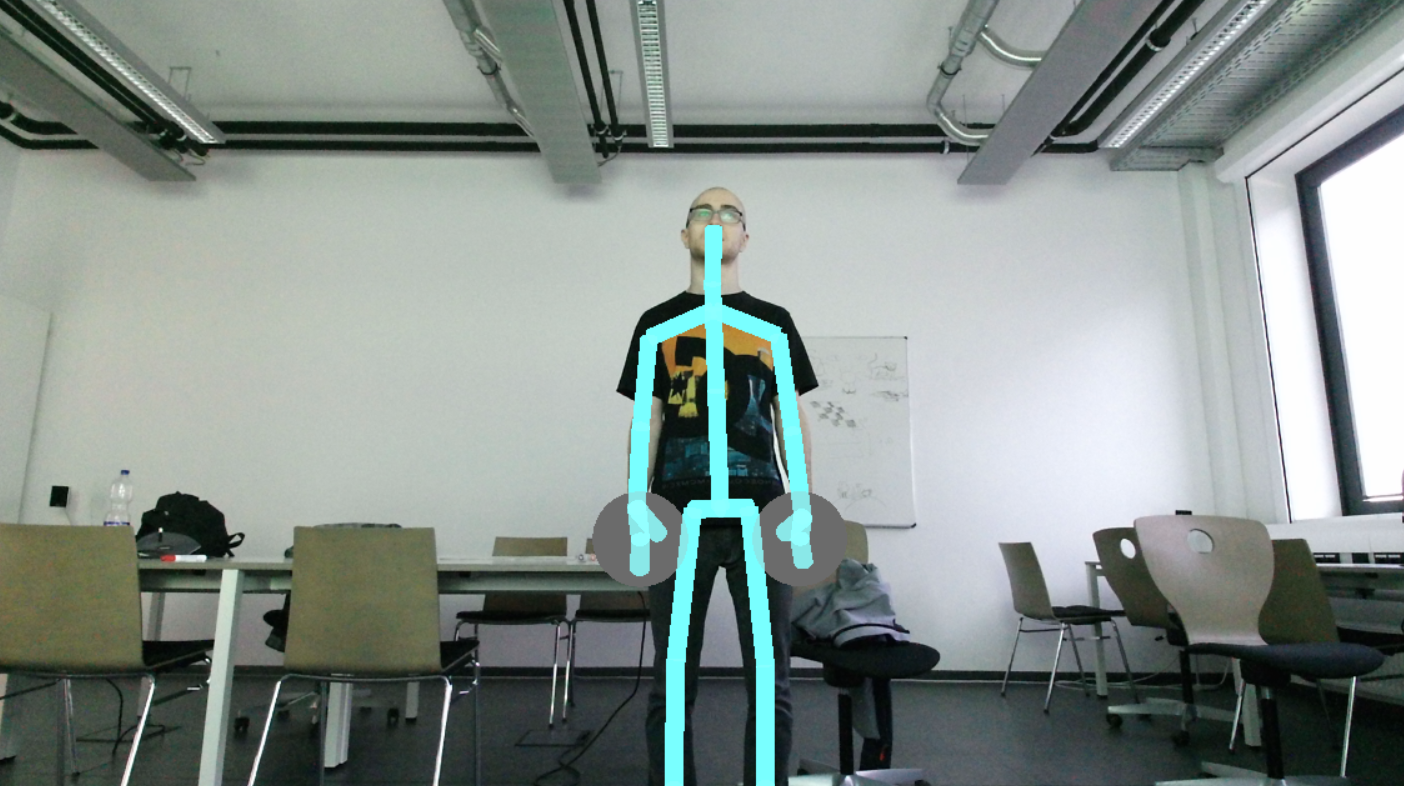
\includegraphics[width=.8\textwidth]{pictures/standardpose_.png}
		\caption{Die Standardpose, in der sich eine Person befinden muss, damit sie vermessen werden kann.}\label{fig:standardp}
		\end{figure}
Aus diesem Grund wird die Vermessung einer Person nur durchgeführt, wenn sich die entsprechende Person über eine bestimmte Anzahl von Frames (etwa 20) durchgehend in der festgelegten Standard-Pose befindet. Weiterhin wird darauf geachtet, dass alle für die Vermessung relevanten Körperproportionen mit ausreichender Konfidenz von der Kinect getrackt werden. Die Kinect liefert hierfür für jeden Skelettpunkt einen von drei möglichen Konfidenzwerten, der angibt, wie warscheinlich die von der Kinect gelieferte Koordinatenwerte für diesen Punkt dem tatsächlichem Wert entsprechen. (Die drei Konfidenzwerte heißen TRACKED, INFERRED, NOT\_TRACKED; wobei TRACKED die höchste Konfidenz und NOT\_TRACKED die niedrigste Konfidenz für einen Skelettpunkt bezeichnet). Ist in einem Frame der Konfidenzwert von einem der beiden Skelettpunkte aus denen eine Körperproportion berechnet wird nicht TRACKED, so wird diese Körperproportion für diesen Frame nicht berücksichtigt bzw. mit Null gewichtet. \par
Eingebettet in unsere Hauptschleife geht die Master-Identifikation folgendermassen von statten: Beim Start des Programms, ist zunächst einmal die Person Master die bzgl. der Kinect die geringste z-Koordinate aufweist. Hierfür wird bei jedem Schleifendurchlauf abgefragt, welche der 6 (potenziell) getrackten Personen, den geringsten z-Wert hat. Der Master wird somit bei jedem Frame neu bestimmt. Durch die Betätigung einer vorher festgelegten Taste wird schließlich die Master-Festlegung auf eine bestimmte Person aktiviert. Hierzu werden die Körperproportionen des bisherigen Masters (d.h. der Person mit dem geringsten z-Wert), über mehrere Frames aus den Skelettdaten extrahiert, gepuffert und schließlich aus diesen für jedes Körpermerkmal der Mittelwert sowie die Standardabweichung berechnet.
	
	
	